%=============================================================================
% Neural Networks and Deep Learning -- Course Project
% Human Activity Recognition from Wi-Fi CSI Doppler spectrograms
%
% Root file. Structured after the NNDL project report template:
%   % !TEX root = report.tex

\section{Introduction}
\label{sec:introduction}

Contactless sensing of human activity is valuable in healthcare, security and
ambient monitoring. Commodity Wi-Fi devices can be repurposed as radar-like
sensors: as a person moves, their body induces micro-Doppler shifts on the
Wi-Fi signal that are captured in the channel-state information (CSI) estimated
by the receiver, \emph{without recording any video}. After suitable processing,
the CSI can be turned into a \emph{Doppler spectrogram}---a
time$\,\times\,$velocity image---whose appearance changes markedly with the
activity being performed, so the recognition problem can be cast as image
classification with a convolutional neural network (CNN)~\cite{sharp}.

The central difficulty is \emph{generalization}. Different people move
differently, and different rooms (and even the same room on different days)
distort the signal differently, so a model that classifies perfectly in its
training environment may collapse on a new one. This is the challenge raised in
the project proposal, which explicitly suggests a
\emph{contrastive / self-supervised} approach to obtain subject- and
environment-independent features. Prior systems close this gap mostly through
signal processing---robust phase sanitization and multi-antenna fusion---at the
cost of a heavy, hand-engineered pipeline~\cite{sharp}; we instead ask how far a
purely \emph{representation-learning} remedy can go on top of a minimal
front-end.

In this report we tackle five-class Wi-Fi HAR under a strict cross-domain
protocol (train on a single environment, test on six unseen ones) and study
whether Supervised Contrastive Learning (SupCon)~\cite{supcon} can \emph{learn}
environment invariance rather than engineering it. The approach is
data-efficient---it reuses the same small training set and a lightweight
encoder---and its value is that the learned features can be reused by any
downstream classifier and combined with the orthogonal signal-processing tools
of the reference system. The report is organized around two clearly separated
contributions:
\begin{itemize}
  \item \textbf{Baseline (M.~Carraro).} A faithful reimplementation, in plain
  PyTorch, of the dataset pipeline and of the baseline Inception-style CNN, with
  a cross-domain evaluation protocol (train on $S1$, test on $S2$--$S7$) and a
  per-measurement-set error breakdown.
  \item \textbf{Contrastive extension (F.~Vezzani).} A Supervised Contrastive
  Learning stage (notebook~\S9): a deeper batch-normalized encoder is pre-trained
  with a supervised-contrastive loss and domain-randomization augmentations to
  learn environment-invariant features, then evaluated with a linear probe under
  the same protocol. It improves cross-domain accuracy over the baseline on
  every set.
\end{itemize}
We use the full SHARP system~\cite{sharp} as the reference upper bound and
discuss, quantitatively, why both of our models sit below it and what the
contrastive stage does and does not recover.

The remainder of the report is structured as follows.
\secref{sec:related_work} reviews the related work on Wi-Fi sensing and
contrastive representation learning. \secref{sec:processing_architecture} gives
a high-level view of the processing pipeline; \secref{sec:model} details the
signals and features, and \secref{sec:learning_framework} describes the two
learning frameworks (baseline CNN and SupCon extension). The experimental
results and the comparison against the SHARP paper are reported in
\secref{sec:results}, and \secref{sec:conclusions} draws the concluding remarks.
 % !TEX root = report.tex

\section{Related Work}
\label{sec:related_work}

\textbf{Wi-Fi sensing and the SHARP system.}
Device-free HAR from commodity Wi-Fi has matured rapidly thanks to the
availability of CSI extraction tools and public datasets. The most relevant work
for us is SHARP~\cite{sharp}, which recognizes human activities from the Doppler
information contained in the CSI of IEEE~802.11ac links and, crucially, targets
\emph{environment and person independence}. SHARP achieves this through two
ingredients: (i) a robust phase-sanitization step that isolates the multipath
components and adopts the \emph{strongest path} as the phase reference, and (ii)
a \emph{decision-fusion} scheme that runs a compact Inception-style CNN on each
of the four receiver antennas and combines the per-antenna decisions. On the
seven measurement sets of the accompanying CSI dataset~\cite{csidataset}, the
full system exceeds $95\%$ accuracy even on rooms, days and persons never seen at
training time. These results are excellent, but they rest on a heavy,
hand-engineered signal-processing front-end; the paper's own ablation shows that
replacing the strongest-path sanitization with the standard reference-antenna
method makes the \emph{same} CNN collapse to $39$--$60\%$ on the unseen sets,
revealing how much of the robustness is carried by the pre-processing rather than
by the learned representation. Our work keeps the minimal front-end (single
antenna, no strongest-path sanitization) and asks how much cross-domain
robustness can instead be recovered on the \emph{representation} side.

\textbf{Contrastive representation learning.}
Contrastive methods learn representations by pulling together ``views'' that
should be similar and pushing apart those that should differ. SimCLR~\cite{simclr}
established a simple self-supervised recipe: two random augmentations of the same
image form a positive pair, all other images in the batch are negatives, and an
encoder is trained with a temperature-scaled InfoNCE loss on $L_2$-normalized
embeddings. Supervised Contrastive Learning (SupCon)~\cite{supcon} extends this
idea to the labelled setting: \emph{all} samples sharing the anchor's label
become positives, which produces tighter, more class-consistent clusters than
cross-entropy and improves robustness to natural corruptions. We adopt SupCon
because its notion of ``positive'' maps naturally onto our goal: two windows of
the same activity should be neighbours \emph{regardless of the environment,
person or antenna they come from}, so that the encoder is driven to discard
domain-specific nuisances. To the best of our knowledge, combining SupCon with
explicit domain-randomization augmentations for cross-domain Wi-Fi HAR on the
SHARP data is the specific extension we contribute here: it complements the
signal-processing route of~\cite{sharp} by attacking domain shift from the
feature-learning side, and we quantify both its gains and its residual limits in
\secref{sec:results}.
 % !TEX root = report.tex

\section{Processing Pipeline}
\label{sec:processing_architecture}

At a high level, both of our models cast Wi-Fi HAR as the classification of
Doppler-spectrogram images and share the \emph{same} data front-end; they differ
only in \emph{how} the representation is learned. \fig{fig:pipeline} sketches the
two chains. Common to both, the raw CSI Doppler traces are cut into fixed-size
windows of shape $1\times340\times100$ (one antenna at a time), which become the
network inputs (\secref{sec:model}). From here the pipeline forks:
\begin{itemize}
  \item the \textbf{baseline chain} (M.~Carraro) feeds each window to an
  Inception-style CNN trained end-to-end with cross-entropy, and reads the
  activity off the softmax output;
  \item the \textbf{contrastive chain} (F.~Vezzani) first applies
  domain-randomization augmentations to build two views of each window, pre-trains
  a deeper batch-normalized encoder with a Supervised Contrastive loss, then
  \emph{freezes} the encoder and fits a linear probe on the resulting features.
\end{itemize}
Both chains are trained on a single environment ($S1$) and evaluated under the
same cross-domain protocol (test on the unseen $S2$--$S7$), so that the two
learning strategies can be compared on equal footing against the reference SHARP
system~\cite{sharp}. The learning frameworks behind the two blocks are detailed
in \secref{sec:learning_framework}.

\begin{figure}[t]
  \centering
  \resizebox{\columnwidth}{!}{%
  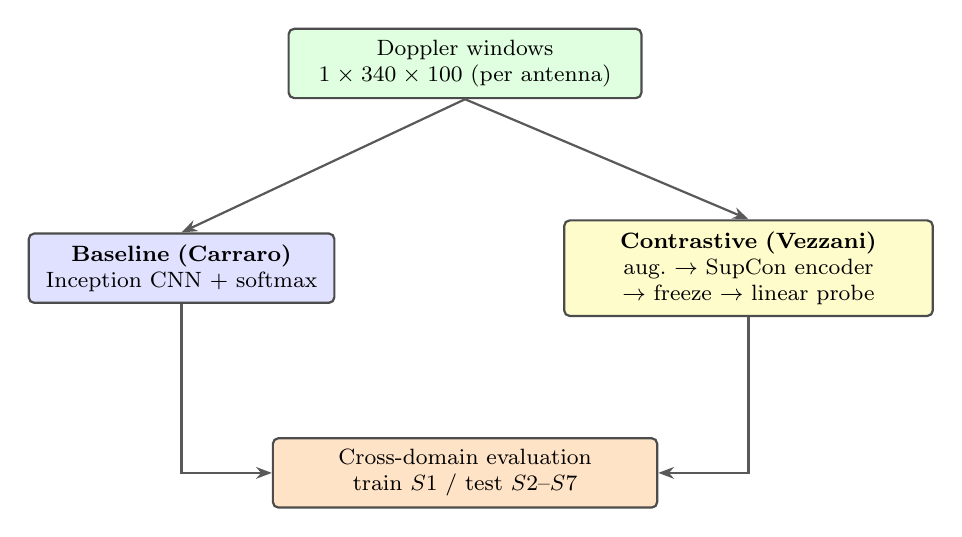
\begin{tikzpicture}[
    font=\footnotesize,
    >={Stealth[length=2mm]},
    box/.style={rectangle, rounded corners=2pt, draw=black!70, thick,
                align=center, inner sep=4pt},
    data/.style={box, fill=green!12, text width=42mm},
    base/.style={box, fill=blue!12, text width=36mm},
    cont/.style={box, fill=yellow!20, text width=44mm},
    eval/.style={box, fill=orange!22, text width=46mm},
    arr/.style={->, thick, black!65},
  ]
    \node[data] (win) at (0,0)
      {Doppler windows\\$1\times340\times100$ (per antenna)};
    \node[base] (bcnn) at (-3.6,-2.6)
      {\textbf{Baseline (Carraro)}\\Inception CNN $+$ softmax};
    \node[cont] (enc) at (3.6,-2.6)
      {\textbf{Contrastive (Vezzani)}\\aug.\ $\to$ SupCon encoder\\$\to$ freeze $\to$ linear probe};
    \node[eval] (ev) at (0,-5.2)
      {Cross-domain evaluation\\train $S1$ / test $S2$--$S7$};

    \draw[arr] (win.south) -- (bcnn.north);
    \draw[arr] (win.south) -- (enc.north);
    \draw[arr] (bcnn.south) |- (ev.west);
    \draw[arr] (enc.south) |- (ev.east);
  \end{tikzpicture}%
  }
  \caption{High-level processing pipeline. A shared front-end turns CSI traces
  into Doppler windows; the baseline chain (M.~Carraro) classifies them directly,
  while the contrastive chain (F.~Vezzani) learns an environment-invariant
  representation before a linear probe. Both are assessed with the same
  cross-domain protocol.}
  \label{fig:pipeline}
\end{figure}

\section{Signals and Features}
\label{sec:model}
\emph{(Dataset pipeline implemented by M.~Carraro.)}

\begin{figure*}[t]
  \centering
  \includegraphics[width=\textwidth]{doppler_activities.png}
  \caption{One example Doppler-spectrogram window per activity (input to the
  network, transposed for readability: rows are the $100$ Doppler-velocity bins,
  columns are the $340$ time samples $\approx 2$\,s). Low-motion classes
  (\emph{empty}, \emph{sitting still}) concentrate energy around zero velocity,
  while \emph{running}/\emph{jumping} spread energy over a wide velocity range.}
  \label{fig:activities}
\end{figure*}

\subsection{The SHARP data}
We use the pre-extracted Doppler traces released with the SHARP
dataset~\cite{csidataset}, collected on IEEE~802.11ac, $80$\,MHz channels. Each
trace is a pickled array of shape $(T,100)$, where $T$ is a variable number of
time steps and $100$ is the number of Doppler-velocity bins, and corresponds to
a single receiving antenna (\texttt{stream\_1}\dots\texttt{stream\_4}) of a
four-antenna monitor.

The recordings map to seven \emph{measurement sets} $S1$--$S7$, each a distinct
(environment, monitor position, person, day) combination
(\tab{tab:conditions}). Only $S1$ is used for training; the others probe
generalization to unseen days ($S2$), unseen persons ($S3$), blocked
line-of-sight ($S4,S5$), a different room ($S6$) and the worst case of
simultaneously new room, day and person ($S7$).

\begin{table}[t]
  \centering
  \caption{Measurement sets of the SHARP dataset (after~\cite{sharp}, Table~1).
  $Mj$: monitor position; $Pi$: person; LOS: direct path present.}
  \label{tab:conditions}
  \begin{tabular}{@{}clllc@{}}
    \toprule
    Set & Monitor & Person & LOS & Role \\
    \midrule
    $S1$ & $M1$ & $P1$ & yes & \textbf{train/val/test} \\
    $S2$ & $M1$ & $P1$ & yes & test (new day) \\
    $S3$ & $M1$ & $P2$ & yes & test (new person) \\
    $S4$ & $M2$ & $P1$ & no  & test (blocked LOS) \\
    $S5$ & $M2$ & $P2$ & no  & test (blocked LOS) \\
    $S6$ & $M3$ & $P1$ & yes & test (new room) \\
    $S7$ & $M4$ & $P3$ & no  & test (all new) \\
    \bottomrule
  \end{tabular}
\end{table}

\subsection{From traces to windows}
To keep the setup comparable across \emph{all} environments, we use the five
core activities present everywhere: \textbf{E} (empty room), \textbf{J}
(jumping), \textbf{L} (sitting still), \textbf{R} (running) and \textbf{W}
(walking), matching the five-class task of the SHARP paper~\cite{sharp}. Each
trace is cut into \emph{non-overlapping} windows of $W_{\text{len}}=340$ time
samples ($\approx 2$\,s); a channel dimension is added, giving inputs of shape
$1\times 340\times 100$. Each of the four antenna streams is treated as an
independent labelled sample: the baseline is therefore a \emph{single-antenna}
classifier that never fuses information across antennas---a point we return to
in \secref{sec:results}. This yields $13{,}564$ windows, reasonably balanced
across classes (E:~$3012$, J:~$2160$, L:~$3056$, R:~$2684$, W:~$2652$).
\fig{fig:activities} shows one window per activity.

\subsection{Cross-domain split}
Following the SHARP protocol, the split is by environment, never random: the
folders of $S1$ ($S1a,S1b,S1c$) are used for training/validation and every other
set is held out for testing; a random split would leak windows from the same
person/room/day into both train and test and overestimate performance. Within
$S1$ we keep $85\%$ for training and $15\%$ for validation (stratified),
giving $2767$ / $489$ / $10{,}308$ windows for train / val / test.

\section{Learning Framework}
\label{sec:learning_framework}

\subsection{Baseline CNN (M.~Carraro)}
\label{sec:baseline}

\begin{figure*}[t]
  \centering
  \resizebox{\textwidth}{!}{%
  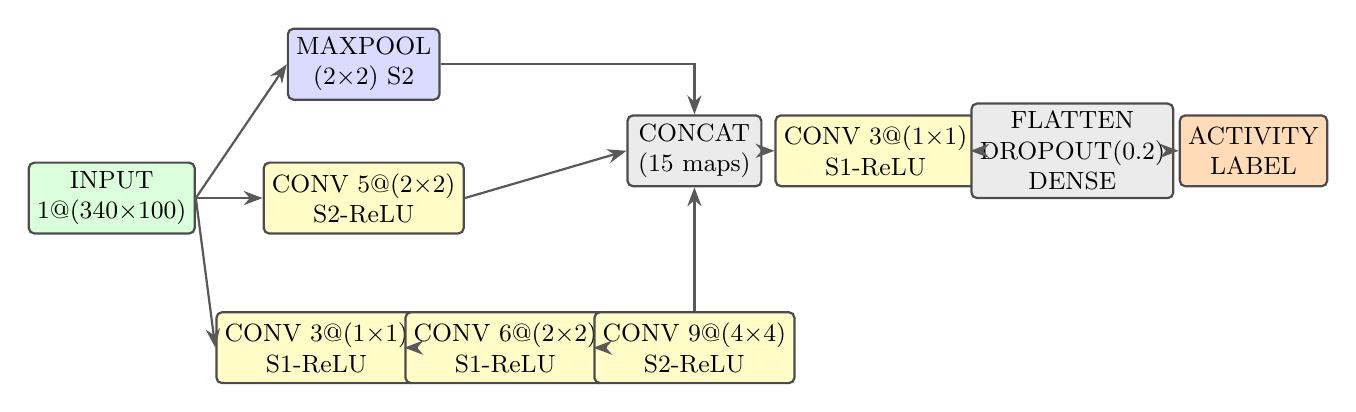
\begin{tikzpicture}[
    font=\small,
    >={Stealth[length=2.4mm]},
    box/.style={rectangle, rounded corners=2pt, draw=black!70, thick,
                align=center, minimum height=9mm, minimum width=17mm, inner sep=3pt},
    input/.style={box, fill=green!14},
    pool/.style={box, fill=blue!14},
    conv/.style={box, fill=yellow!22},
    op/.style={box, fill=black!8},
    term/.style={box, fill=orange!28},
    arr/.style={->, thick, black!65},
  ]
    % input
    \node[input] (in) at (0,0) {INPUT\\1@(340$\times$100)};
    % three branches
    \node[pool] (mp) at (3.2,1.7) {MAXPOOL\\(2$\times$2) S2};
    \node[conv] (b2) at (3.2,0.0) {CONV 5@(2$\times$2)\\S2-ReLU};
    \node[conv] (b3a) at (2.6,-1.9) {CONV 3@(1$\times$1)\\S1-ReLU};
    \node[conv] (b3b) at (5.0,-1.9) {CONV 6@(2$\times$2)\\S1-ReLU};
    \node[conv] (b3c) at (7.4,-1.9) {CONV 9@(4$\times$4)\\S2-ReLU};
    % concat + head
    \node[op]   (cat) at (7.4,0.6) {CONCAT\\(15 maps)};
    \node[conv] (red) at (9.7,0.6) {CONV 3@(1$\times$1)\\S1-ReLU};
    \node[op]   (fc)  at (12.2,0.6) {FLATTEN\\DROPOUT(0.2)\\DENSE};
    \node[term]  (lab) at (14.5,0.6) {ACTIVITY\\LABEL};

    % arrows from input to branches
    \draw[arr] (in.east) -- (mp.west);
    \draw[arr] (in.east) -- (b2.west);
    \draw[arr] (in.east) -- (b3a.west);
    % third branch chain
    \draw[arr] (b3a.east) -- (b3b.west);
    \draw[arr] (b3b.east) -- (b3c.west);
    % branches to concat
    \draw[arr] (mp.east)  -| (cat.north);
    \draw[arr] (b2.east)  -- (cat.west);
    \draw[arr] (b3c.north) -- (cat.south);
    % head
    \draw[arr] (cat.east) -- (red.west);
    \draw[arr] (red.east) -- (fc.west);
    \draw[arr] (fc.east)  -- (lab.west);
  \end{tikzpicture}%
  }
  \caption{Baseline single-antenna classification architecture (M.~Carraro), a
  faithful reproduction of the SHARP reduced-Inception module~(\cite{sharp},
  Fig.~4). Three parallel branches (max-pool / strided conv / three stacked
  convs) extract multi-scale Doppler features; the maps are concatenated
  ($1{+}5{+}9=15$), reduced to $3$ by a $1\times1$ convolution, then flattened and
  classified by a dense layer with dropout ($128{,}535$ parameters). \texttt{S2}
  denotes stride~2; every CONV is followed by a ReLU.}
  \label{fig:baseline_arch}
\end{figure*}

The baseline reproduces the simplified reduced-Inception module of SHARP
(\cite{sharp}, Fig.~4), shown in \fig{fig:baseline_arch}. Three parallel branches
process the $1\times340\times100$ input and produce feature maps of identical
spatial size $170\times50$ so they can be concatenated on the channel axis:
\begin{itemize}
  \item \textbf{Branch 1:} $\mathrm{MaxPool}(2\times2,\ \text{stride }2)$
  $\rightarrow 1$ channel (no parameters);
  \item \textbf{Branch 2:} $\mathrm{Conv}(5,\,2\times2,\ \text{stride }2)+\mathrm{ReLU}$
  $\rightarrow 5$ channels;
  \item \textbf{Branch 3:} $\mathrm{Conv}(3,\,1\times1)\rightarrow
  \mathrm{Conv}(6,\,2\times2,\ \text{pad }2)\rightarrow
  \mathrm{Conv}(9,\,4\times4,\ \text{stride }2)$, each $+\,\mathrm{ReLU}$
  $\rightarrow 9$ channels.
\end{itemize}
The branches are concatenated ($1{+}5{+}9=15$ channels), reduced to $3$ channels
by a $1\times1$ convolution, flattened, passed through $\mathrm{Dropout}(0.2)$
and a final dense layer with one logit per class. The model has
$\mathbf{128{,}535}$ trainable parameters---exactly the count reported for the
SHARP baseline CNN~\cite{sharp}.

Training uses cross-entropy loss and Adam ($\text{lr}=10^{-3}$), mini-batches of
$64$, and \emph{early stopping}: training halts when the validation loss has not
improved for $7$ epochs (budget $40$), and the best (lowest validation-loss)
weights are restored before testing. In our run, training stopped after
epoch~$13$ (best validation loss $0.993$). \fig{fig:curves} shows the loss and
accuracy curves: training accuracy keeps climbing while validation accuracy
plateaus around $0.52$---the classic signature of a model overfitting its single
training environment.

\begin{figure}[t]
  \centering
  \includegraphics[width=\columnwidth]{training_curves.png}
  \caption{Baseline training. Left: cross-entropy loss; right: accuracy.
  Validation accuracy plateaus near $0.52$ while training accuracy keeps rising,
  i.e.\ the model overfits the single training set $S1$; early stopping halts
  training at epoch~13.}
  \label{fig:curves}
\end{figure}

\subsection{Contrastive extension: Supervised Contrastive Learning (F.~Vezzani)}
\label{sec:contrastive}
\emph{(Developed by F.~Vezzani; implemented and trained as Section~9 of the
notebook.)}

\subsubsection{Motivation}
The baseline is trained with plain cross-entropy on a single environment, so
nothing pushes its features to be invariant across domains. Following the
\emph{contrastive / self-supervised} direction suggested in the project
proposal, we implement \emph{Supervised Contrastive Learning}
(SupCon)~\cite{supcon}. The key change is \emph{what} is optimized: instead of
predicting the label directly, an \emph{encoder} is first trained so that two
windows of the \emph{same activity} are pulled together and windows of different
activities are pushed apart---\emph{regardless of the environment, person or
antenna they come from}. Because the objective depends only on activity
identity, the encoder is encouraged to discard environment-specific nuisances. A
tiny linear classifier is then fit on top of the frozen representation
(\emph{linear probe}).

\subsubsection{Domain-randomization augmentations}
SupCon needs, for each window, two augmented ``views'' that keep the activity
intact but perturb nuisance factors, acting as a light domain randomization
(\fig{fig:aug}). All transforms run on-GPU on a whole batch (default
parameters in parentheses):
\begin{itemize}
  \item \textbf{amplitude scaling} by a per-window random gain
  ($\mathcal{U}(0.8,1.2)$)---rooms/distances reflect the signal with different
  strength;
  \item \textbf{additive Gaussian noise} ($\sigma=0.05$);
  \item \textbf{circular time shift} ($\pm 40$ samples)---the activity does not
  depend on where in the $\approx 2$\,s window it starts;
  \item \textbf{time and Doppler masking} (SpecAugment-style: a zeroed band of
  $40$ time samples and $15$ velocity bins)---forces the encoder to use the whole
  time--velocity pattern rather than any single region.
\end{itemize}

\begin{figure}[t]
  \centering
  \includegraphics[width=\columnwidth]{augment_views.png}
  \caption{A window (\emph{left}) and two augmented views. Amplitude scaling and
  Gaussian noise change the texture; the circular time shift and the
  SpecAugment-style time/Doppler masks (dark bands) hide parts of the pattern,
  while the activity signature (the horizontal energy band) is preserved.}
  \label{fig:aug}
\end{figure}

\subsubsection{Encoder and projection head}
The encoder $f(\cdot)$ is a deeper, batch-normalized evolution of the baseline's
Inception block (\tab{tab:encoder}). It keeps the three-branch Inception
front-end (max-pool / strided conv / deeper conv, concatenated to $41$ channels)
but adds (i) batch normalization after every convolution, (ii) a $1\times1$
channel-mixing reduction to $32$ channels, (iii) a second downsampling stage
($32\!\rightarrow\!64\!\rightarrow\!128$), and (iv) \emph{global average
pooling}, replacing the baseline's large \texttt{flatten}$\rightarrow$dense layer
with a fixed $128$-dimensional representation $h$ that has fewer parameters and
is more shift-robust. A small MLP \emph{projection head} $g(\cdot)$
($128\!\rightarrow\!128\!\rightarrow\!128$, ReLU) maps $h$ to an
$L_2$-normalized embedding $\bm{z}=g(h)$ on the unit hypersphere; as prescribed by
SupCon, the loss is applied to $\bm{z}$ and the head is \emph{discarded} after
pre-training, so classification uses $h$. The whole model has $130{,}952$
parameters (encoder $\approx\!97.9$k $+$ head $\approx\!33$k), comparable to the
baseline's $128.5$k.

\begin{table}[t]
  \centering
  \caption{Contrastive encoder $f(\cdot)$; output sizes for a
  $1\times340\times100$ input. BN$+$ReLU follow every convolution; ``sN''
  denotes stride~N (default stride~1). The pooling output is the $128$-d
  representation $h$.}
  \label{tab:encoder}
  \setlength{\tabcolsep}{4pt}
  \begin{tabular}{@{}lll@{}}
    \toprule
    Stage & Layers & Output ($C\times H\times W$) \\
    \midrule
    Inception & maxpool(2); conv(16,s2); & $41\times170\times50$\\
              & conv(16)$\rightarrow$conv(24,s2) & \\
    Reduce    & conv(32,\,$1\times1$) & $32\times170\times50$\\
    Stage 2   & conv(64,s2)$\rightarrow$conv(128,s2) & $128\times43\times13$\\
    Pool      & global average pool & $128$\\
    \bottomrule
  \end{tabular}
\end{table}

\subsubsection{SupCon loss}
For a batch of $L_2$-normalized embeddings with labels, each anchor $i$ attracts
every other sample sharing its label (its positive set $P(i)$) and repels all
others, through a temperature-scaled softmax over cosine similarities:
\begin{equation}
\label{eq:supcon}
\mathcal{L}=\frac{1}{|I|}\sum_{i\in I}\frac{-1}{|P(i)|}\sum_{p\in P(i)}
\log\frac{\exp(\bm{z}_i\!\cdot\!\bm{z}_p/\tau)}
{\sum_{a\neq i}\exp(\bm{z}_i\!\cdot\!\bm{z}_a/\tau)},
\end{equation}
where $I$ is the set of anchors with at least one same-class positive (the
implementation averages the per-anchor terms over the batch) and the temperature
is $\tau=0.07$. Unlike self-supervised SimCLR~\cite{simclr}, using the labels in
\eq{eq:supcon} makes \emph{all} same-activity windows in the batch positives---even
those from different files or environments---which turns generic contrastive
learning into an environment-invariant \emph{activity} representation.

\subsubsection{Training and evaluation protocol}
Everything uses the \emph{same} $S1$-based split as the baseline.
\begin{itemize}
  \item \textbf{Contrastive pre-training.} Each batch is expanded into two
  augmented views; encoder and head are trained jointly with Adam
  (lr~$10^{-3}$, weight decay~$10^{-4}$) for up to $30$ epochs with early
  stopping (patience~$7$) on the validation contrastive loss, keeping the best
  encoder.
  \item \textbf{Linear probe.} The encoder is frozen, embeddings are
  pre-computed and standardized with training statistics, and a single
  $\mathrm{Linear}(128,5)$ layer is trained with cross-entropy (Adam,
  lr~$10^{-3}$, early stopping). This isolates the quality of the representation.
  \item \textbf{Optional fine-tuning.} The encoder is then unfrozen and the full
  network fine-tuned end-to-end with a small learning rate ($10^{-4}$).
\end{itemize}
The model is evaluated under the same cross-domain protocol as the baseline
(train on $S1$, test on $S2$--$S7$). A t-SNE projection of the test embeddings,
colored by activity and by environment, is used as a diagnostic of
environment-invariance.
 % !TEX root = report.tex

\section{Results}
\label{sec:results}

All numbers come from the stored notebook outputs, one run per configuration,
under the same protocol: train on $S1$, test on the unseen $S2$--$S7$.
\tab{tab:compare} collects them per measurement set and \fig{fig:perset} plots
the four milestones; \tab{tab:versions} maps each column to the change that
produced it.

\subsection{Baseline}
On the pooled unseen test set the baseline reaches $\mathbf{48.2\%}$ accuracy
(test loss $1.052$), from $45.5\%$ ($S2$) to $52.3\%$ ($S7$). Its confusion matrix
(\fig{fig:cm}\,(a)) shows two dominant error modes: \emph{sitting still} is
absorbed by \emph{empty} ($L\!\rightarrow\!E$: $0.76$), both being near-static and
concentrated at zero Doppler velocity, and \emph{running}/\emph{walking} are
heavily confused with each other ($0.39$ and $0.28$).

\subsection{Contrastive representation}
The linear probe on the frozen SupCon encoder raises overall accuracy to
$\mathbf{53.1\%}$ (validation $58.3\%$): $+4.9$ points, and an improvement on
\emph{every} set, the largest on $S3$ ($+8.3$, unseen person) and $S7$ ($+5.9$,
all conditions new). Its confusion matrix (\fig{fig:cm}\,(b)) sharpens
\emph{running} and softens the $L\!\rightarrow\!E$ confusion
($0.76\!\rightarrow\!0.52$). \emph{End-to-end fine-tuning} then \emph{hurts},
dropping back to $48.4\%$: freezing the pre-trained encoder is what generalizes,
while fine-tuning re-overfits the single training environment.

The t-SNE projection (\fig{fig:tsne}, from the sliding-window run of
\secref{sec:sliding}) is the most informative diagnostic. Colored by
\emph{environment} (right) the points are thoroughly mixed---the
SupCon objective \emph{did} reach its design goal of an environment-invariant
representation. Colored by \emph{activity} (left) the space splits into a
static region (\emph{empty}, \emph{sitting}) and a moving arc (\emph{jumping},
\emph{running}, \emph{walking}), but the activities \emph{within} each region
stay partly entangled: contrastive learning removed the \emph{domain} nuisance
and exposed a harder, intrinsic limit---a single-antenna $\approx\!2$\,s window
does not fully separate the activities, whichever way it is encoded.
Consistently, in both runs the SupCon loss fell only from $\approx\!4.6$ to
$\approx\!4.3$: the pre-training never fully converged.

\begin{figure*}[t]
  \centering
  \begin{subfigure}{0.245\textwidth}
    \includegraphics[width=\textwidth]{confusion_overall_c.png}
    \caption{baseline, non-overlapping}
  \end{subfigure}\hfill
  \begin{subfigure}{0.245\textwidth}
    \includegraphics[width=\textwidth]{cl_confusion_c.png}
    \caption{$+$ SupCon linear probe}
  \end{subfigure}\hfill
  \begin{subfigure}{0.245\textwidth}
    \includegraphics[width=\textwidth]{confusion_v4_single_c.png}
    \caption{baseline, sliding window}
  \end{subfigure}\hfill
  \begin{subfigure}{0.245\textwidth}
    \includegraphics[width=\textwidth]{confusion_v4_fused_c.png}
    \caption{$+$ $4$-antenna fusion}
  \end{subfigure}
  \caption{Row-normalized confusion matrices on all unseen test environments,
  along the four milestones of \fig{fig:perset}. The contrastive representation
  (b) softens the $L\!\rightarrow\!E$ confusion of the baseline (a); the sliding
  window (c) lifts every class; fusion (d) then repairs the low-motion pair
  itself, $L$ going from $0.50$ to $0.75$ correct with the \emph{same} weights.}
  \label{fig:cm}
\end{figure*}

\begin{figure}[t]
  \centering
  \includegraphics[width=\columnwidth]{tsne_slide.png}
  \caption{t-SNE of the test embeddings of the SupCon encoder (sliding-window
  run). \emph{Left},
  colored by activity: a static region (\emph{empty}, \emph{sitting}) and a
  moving arc (\emph{jumping}, \emph{running}, \emph{walking}). \emph{Right}, the
  same points colored by environment: the colors are mixed \emph{inside} the
  structure, i.e.\ the space is organized by \emph{activity}, not by
  \emph{environment}.}
  \label{fig:tsne}
\end{figure}

\subsection{Optimizer schedule}
The slow schedule changes only the learning rate, the patience and the epoch
budget, so the two runs isolate that factor. Slowing
training down \emph{improves} cross-domain accuracy from $48.2\%$ to $51.3\%$
($+3.1$ points, five sets out of six) even though the model fits its own training
data \emph{worse} ($0.575$ vs.\ $0.601$, \fig{fig:curves}). With a single
training environment the two objectives conflict: an epoch spent fitting $S1$
better is also an epoch spent memorizing its room, person and day. It also
tempers the previous subsection---$+3.1$ of the contrastive model's $+4.9$ points
can be bought with an optimizer setting alone, so single-run gains of a few
points here are fragile.

\subsection{Sliding-window front-end}
\label{sec:sliding}
Cutting the same recordings at stride $30$ instead of $340$ turns $13{,}564$
windows into $152{,}320$ and takes the \emph{unchanged} architecture from
$48.2\%$ to $\mathbf{59.3\%}$ ($+11.1$ points), improving every measurement set
by $8.4$ to $15.3$ points. Two caveats keep this honest: the run also raises the
early-stopping patience from $7$ to $12$, so a small part of the gain belongs to
the longer schedule; and the extra windows are strongly
correlated, so the effective sample size grows far less than tenfold. The cost is
real---$\approx\!21$\,GB of resident memory and an epoch an order of magnitude
slower, which is exactly why the loader had to allocate once instead of
concatenating---but the payoff is the single largest gain from the data side, and
it confirms that the reference implementation's stride is not an arbitrary
choice. \fig{fig:curves}(c) shows the model now reaching $0.756$ training
accuracy with validation accuracy $12$ points above the non-overlapping run, i.e.\
the denser windows buy genuine fitting capacity rather than only noise.

\subsection{Multi-antenna decision fusion}
Averaging the four per-antenna probability vectors (\eq{eq:fusion}) is the
largest single improvement we measured, and it is free: no retraining, no extra
parameters, one softmax and one group-average at inference. On the
sliding-window model it lifts $59.3\%$ to $\mathbf{72.1\%}$ ($+12.8$ points, from
$+6.9$ on $S7$ to $+17.1$ on $S2$); on the non-overlapping model it gave $+10.2$
($51.3\!\rightarrow\!61.5\%$). The gain is therefore robust to the data regime.

Its mechanism, though, changes with that regime. At stride $340$
(\tab{tab:compare}) fusion sharpened the motion classes but left
\emph{sitting}$\rightarrow$\emph{empty} untouched: with almost no motion in a
window the four antennas simply agreed on the same wrong answer. At stride $30$
the single-antenna model is already half-right on that pair
(\fig{fig:cm}\,(c), $L$ at $0.50$), and fusion converts it into the largest
per-class gain of all---$L$ reaches $0.75$ and $L\!\rightarrow\!E$ falls from
$0.45$ to $0.23$ (\fig{fig:cm}\,(d))---alongside \emph{jumping}
($0.56\!\rightarrow\!0.72$) and \emph{running} ($0.63\!\rightarrow\!0.75$).
Averaging only helps where the individual antennas disagree; denser temporal
coverage is what creates that disagreement on low-motion windows.

\begin{figure}[t]
  \centering
  \includegraphics[width=\columnwidth]{perset_accuracy.png}
  \caption{Cross-domain accuracy per measurement set along the four milestones
  (dashed line: the $20\%$ chance level). Every unseen set benefits from the
  sliding window and, on top of it, from antenna fusion.}
  \label{fig:perset}
\end{figure}

\subsection{Does contrastive learning still help?}
Repeating the contrastive stage on the sliding-window data answers a question the
first experiment could not: the linear probe now reaches $58.3\%$, i.e.\ $1.0$
point \emph{below} the plain baseline it beat by $4.9$ points in the data-poor
regime, and fine-tuning again does worse ($57.0\%$). Read together with
\tab{tab:compare}, the contrastive stage behaves as a \emph{data-efficiency}
mechanism rather than a domain-invariance mechanism per se: when only $2767$
training windows are available it buys a representation that plain cross-entropy
cannot learn, and when $31{,}103$ (correlated) windows are available
cross-entropy catches up on its own. One confound deserves mention: the
contrastive and probe learning rates were left at $10^{-4}$ in that run while the
baseline used $10^{-3}$, so part of the one-point deficit may be an under-trained
encoder rather than the data regime.

\subsection{Comparison with the SHARP paper}
\tab{tab:compare} places our results next to the SHARP paper~\cite{sharp}: the
\emph{full} system (strongest-path sanitization $+$ 4-antenna fusion) and an
\emph{ablation} that swaps the strongest-path sanitization for the standard
reference-antenna method, feeding the \emph{same} CNN (\cite{sharp}, Table~4).
Full SHARP stays above $95\%$ everywhere. Our best configuration
(sliding window $+$ fusion, $72.1\%$) beats the ablation on \emph{every} unseen
set, by $10.6$ points ($S7$) to $26.8$ points ($S5$), and its margin is largest
exactly where the ablation collapses---the blocked-line-of-sight sets $S4$ and
$S5$. The residual $\sim\!26$-point gap to full SHARP is thus concentrated in the
one ingredient we do not implement, the strongest-path phase sanitization. The
acquisition campaigns behind the dataset also spanned nearly two years
(\cite{sharp}, Sec.~5.2), and that time diversity is itself part of what the
reference results build on.

\begin{table*}[t]
  \centering
  \caption{Per-set accuracy (\%), training on $S1$ and testing on the unseen
  sets, one run per column. Non-overlapping windows: baseline under the fast
  ($10^{-3}$) and slow ($10^{-4}$) schedules, SupCon linear probe, and fusion on
  the slow-schedule model. Sliding window (stride $30$): baseline, SupCon probe
  and fusion. Fusion always re-uses the weights of the baseline to its left.
  SHARP columns from~\cite{sharp} (Tables~3 and~4).}
  \label{tab:compare}
  \setlength{\tabcolsep}{5pt}
  \small
  \begin{tabular}{@{}lcccccccccc@{}}
    \toprule
     & \multicolumn{4}{c}{\textbf{Non-overlapping windows}}
     & \multicolumn{3}{c}{\textbf{Sliding window (stride 30)}}
     & \multicolumn{2}{c}{\textbf{SHARP~\cite{sharp}}}\\
    \cmidrule(lr){2-5}\cmidrule(lr){6-8}\cmidrule(lr){9-10}
    Set & Base (fast) & SupCon & Base (slow) & $+$ Fusion
        & Base & SupCon & $+$ Fusion & Full & Abl.\\
    \midrule
    $S2$ & $45.5$ & $51.1$ & $50.9$ & $62.6$ & $60.8$ & $59.3$ & $77.9$ & $99.8$ & $59.8$\\
    $S3$ & $51.4$ & $59.7$ & $55.9$ & $68.8$ & $61.6$ & $61.5$ & $75.2$ & $99.3$ & $58.0$\\
    $S4$ & $48.5$ & $51.9$ & $50.6$ & $58.1$ & $56.9$ & $55.6$ & $66.2$ & $97.6$ & $43.5$\\
    $S5$ & $47.5$ & $52.9$ & $49.8$ & $57.5$ & $57.4$ & $55.3$ & $66.0$ & $96.6$ & $39.2$\\
    $S6$ & $48.1$ & $51.3$ & $50.6$ & $57.9$ & $57.4$ & $56.5$ & $72.7$ & $99.8$ & $59.4$\\
    $S7$ & $52.3$ & $58.2$ & $51.5$ & $68.9$ & $64.0$ & $65.3$ & $70.9$ & $96.0$ & $60.3$\\
    \midrule
    \textbf{Overall} & $48.2$ & $53.1$ & $51.3$ & $61.5$ & $59.3$ & $58.3$ &
    $\mathbf{72.1}$ & $\sim\!98$ & $\sim\!53$\\
    \bottomrule
  \end{tabular}
\end{table*}

\subsection{Discussion}
\label{sec:discussion}

\paragraph{What each change bought}
Ranked by measured effect, decision fusion ($+12.8$) and the sliding window
($+11.1$) dominate the contrastive representation ($+4.9$, and $-1.0$ once data
is plentiful) and the optimizer schedule ($+3.1$). The ordering is a finding in
itself: the two cheapest changes---a stride constant and a few lines of
post-processing over information already present in the dataset---beat the one
that cost the most design effort, and they compose, taking the \emph{same}
$128{,}535$-parameter network from $48.2\%$ to $72.1\%$. It also matches SHARP's
own ablation, where accuracy grows monotonically with the number of fused
antennas~\cite{sharp}.

\paragraph{Why we are still far from SHARP}
The gap is now essentially one component. SHARP uses the \emph{strongest}
multipath component as phase reference, and its ablation shows the standard
reference-antenna method makes the \emph{same} CNN collapse from $>95\%$ to
$39$--$60\%$ (\tab{tab:compare}, last column). Our best model sits $10$ to $27$
points \emph{above} that ablation, so we have reproduced the decision-level half of
SHARP's robustness and improved on the data side, but none of its
signal-processing half. Training on one small environment also makes every number
high-variance.

\paragraph{Where representation learning fits}
The SupCon stage attacks domain shift on the \emph{representation} axis and, as
the t-SNE shows, succeeds there; but its measured advantage evaporates when the
front-end supplies ten times more windows. The practical reading is that
contrastive pre-training is worth its complexity when labelled windows are
scarce---which is the realistic setting for a new deployment with one calibration
environment---while in the data-rich regime the effort is better spent on the
front-end and on the decision rule. The experiment left undone is fusion on top
of the frozen probe with the contrastive stage re-tuned at $10^{-3}$: all the
components exist in the released code, but no run combines them.
 % !TEX root = report.tex

\section{Concluding Remarks}
\label{sec:conclusions}

We reproduced and evaluated a baseline Wi-Fi HAR pipeline under a strict
cross-domain protocol ($48.2\%$ on unseen environments) and added a Supervised
Contrastive Learning extension that improves cross-domain accuracy on every
measurement set ($53.1\%$ overall, $+4.9$ points). A t-SNE analysis shows that
the extension achieves its intended goal---an environment-invariant
representation---while a direct comparison with the SHARP paper~\cite{sharp}
places both models well below the full pipeline, whose multi-antenna decision
fusion and strongest-path phase sanitization we do not implement.

The practical value of the extension is that it recovers domain robustness
\emph{on the learning side}, with a lightweight encoder, no extra
signal-processing, and a frozen, reusable feature space. Since its residual
errors are \emph{activity} confusions rather than \emph{domain} shift, the
contrastive encoder is complementary to SHARP's antenna fusion: the clearest next
step is to combine the two---keeping the frozen encoder---ideally with a
sliding-window dataset and multi-seed runs.

\paragraph{What we learned and difficulties encountered}
The main lesson was that a strict, environment-based split changes the story:
modest-looking numbers ($\sim\!50\%$) are the honest cost of never seeing the
test environment, which a random split would have hidden. The t-SNE proved
valuable as a diagnostic---it revealed that contrastive learning had solved the
\emph{domain} axis but not the \emph{activity} axis. The main difficulties were:
(i) getting SupCon pre-training to converge (the loss barely moved), so the
representation is useful but under-trained; (ii) the counter-intuitive finding
that end-to-end fine-tuning \emph{hurt} generalization by re-overfitting the
single environment, which taught us to trust the frozen-encoder / linear-probe
evaluation; and (iii) the high run-to-run variance of the small baseline, which
makes single-run comparisons fragile and calls for multi-seed averaging.

%
% Authors / contributions:
%   * Marco Carraro     -- dataset pipeline + baseline CNN
%   * Francesco Vezzani -- Supervised Contrastive Learning extension
%
% Compile with pdflatex + bibtex (IEEEtran.cls is bundled in this folder).
%=============================================================================
\documentclass[10pt, conference, letterpaper]{IEEEtran}

\usepackage{amsmath}
\usepackage{amssymb}
\usepackage{amsfonts}
\usepackage{mathtools}
\usepackage[utf8]{inputenc}
\usepackage{xcolor}
\usepackage{graphicx}
\usepackage{caption}
\usepackage{subcaption}
\usepackage{booktabs}
\usepackage{array}
\usepackage{cite}
\usepackage{bm}
\usepackage{tikz}
\usetikzlibrary{arrows.meta,positioning,fit,backgrounds,calc}

% IEEEtran defaults the typewriter face to Courier (pcr); use the always-available
% Computer Modern typewriter instead so the report builds on any TeX install.
\renewcommand{\ttdefault}{cmtt}

\renewcommand{\thetable}{\arabic{table}}
\renewcommand{\thesubtable}{\alph{subtable}}

\DeclareMathOperator*{\argmin}{arg\,min}
\DeclareMathOperator*{\argmax}{arg\,max}

\graphicspath{{./figures/}}
\setlength{\belowcaptionskip}{0mm}
\setlength{\textfloatsep}{6pt}
\setlength{\dbltextfloatsep}{6pt}
\setlength{\intextsep}{6pt}
\setlength{\abovecaptionskip}{2pt}
\captionsetup{font=footnotesize}

% ---- Cross-referencing helpers (as in the template) -------------------------
\newcommand{\eq}[1]{Eq.~\eqref{#1}}
\newcommand{\fig}[1]{Fig.~\ref{#1}}
\newcommand{\tab}[1]{Tab.~\ref{#1}}
\newcommand{\secref}[1]{Section~\ref{#1}}
\newcommand{\rev}[1]{{\color{blue}#1}}
\newcommand{\red}[1]{{\color{red}#1}}
\newcommand{\mytexttilde}{{\raise.17ex\hbox{$\scriptstyle\mathtt{\sim}$}}}

\setlength{\columnsep}{0.2in}
\IEEEoverridecommandlockouts

\begin{document}

\title{Human Activity Recognition from Wi-Fi CSI Doppler Spectrograms:\\
A CNN Baseline and a Contrastive Extension for Cross-Domain Generalization}

\author{\; \qquad Marco Carraro$^\dag$ \quad \; Francesco Vezzani$^\dag$
\thanks{$^\dag$Department of Information Engineering, University of Padova, Italy, \newline
email: \texttt{marco.carraro.23@studenti.unipd.it}, [Mat. 2159568]\newline
email: \texttt{francesco.vezzani.1@studenti.unipd.it}, [Mat. 2159567]}
}

\maketitle

%=============================================================================
\begin{abstract}
We study device-free human activity recognition (HAR) from the Doppler
spectrograms of Wi-Fi channel-state information (CSI), using the
released traces of the SHARP dataset~\cite{sharp,csidataset}. Starting from the
Inception-style convolutional baseline, trained
only on measurement set~$S1$ and evaluated on the six unseen sets
$S2$--$S7$. We add and measure, one change at a time, four strategies for
closing the cross-domain gap without the hand-engineered front-end of the
reference system: (i) supervised contrastive pre-training, with a linear probe
on the frozen representation; (ii) a slower optimizer schedule; (iii) an
overlapping sliding window at the stride used by the dataset authors and (iv) 
multi-antenna soft
decision fusion, averaging the per-antenna probability vectors of each
physical time window with no retraining and no extra parameters. The last two
compose into our best configuration, taking the same network from
$48.2\%$ to $\mathbf{72.7\%}$ and beating the single-component ablation of the
reference system on every unseen set. Contrastive pre-training helps in the
data-poor regime but stops helping once the sliding window supplies
substantially more training windows. The residual gap to the full reference
pipeline is attributable to its strongest-path phase sanitization, which we
do not implement.
\end{abstract}

% !TEX root = report.tex

\section{Introduction}
\label{sec:introduction}

Contactless sensing of human activity is valuable in healthcare, security and
ambient monitoring. Commodity Wi-Fi devices can be repurposed as radar-like
sensors: as a person moves, their body induces micro-Doppler shifts on the
Wi-Fi signal that are captured in the channel-state information (CSI) estimated
by the receiver, \emph{without recording any video}. After suitable processing,
the CSI can be turned into a \emph{Doppler spectrogram}---a
time$\,\times\,$velocity image---whose appearance changes markedly with the
activity being performed, so the recognition problem can be cast as image
classification with a convolutional neural network (CNN)~\cite{sharp}.

The central difficulty is \emph{generalization}. Different people move
differently, and different rooms (and even the same room on different days)
distort the signal differently, so a model that classifies perfectly in its
training environment may collapse on a new one. This is the challenge raised in
the project proposal, which explicitly suggests a
\emph{contrastive / self-supervised} approach to obtain subject- and
environment-independent features. Prior systems close this gap mostly through
signal processing---robust phase sanitization and multi-antenna fusion---at the
cost of a heavy, hand-engineered pipeline~\cite{sharp}; we instead ask how far a
purely \emph{representation-learning} remedy can go on top of a minimal
front-end.

In this report we tackle five-class Wi-Fi HAR under a strict cross-domain
protocol (train on a single environment, test on six unseen ones) and study
whether Supervised Contrastive Learning (SupCon)~\cite{supcon} can \emph{learn}
environment invariance rather than engineering it. The approach is
data-efficient---it reuses the same small training set and a lightweight
encoder---and its value is that the learned features can be reused by any
downstream classifier and combined with the orthogonal signal-processing tools
of the reference system. The report is organized around two clearly separated
contributions:
\begin{itemize}
  \item \textbf{Baseline (M.~Carraro).} A faithful reimplementation, in plain
  PyTorch, of the dataset pipeline and of the baseline Inception-style CNN, with
  a cross-domain evaluation protocol (train on $S1$, test on $S2$--$S7$) and a
  per-measurement-set error breakdown.
  \item \textbf{Contrastive extension (F.~Vezzani).} A Supervised Contrastive
  Learning stage (notebook~\S9): a deeper batch-normalized encoder is pre-trained
  with a supervised-contrastive loss and domain-randomization augmentations to
  learn environment-invariant features, then evaluated with a linear probe under
  the same protocol. It improves cross-domain accuracy over the baseline on
  every set.
\end{itemize}
We use the full SHARP system~\cite{sharp} as the reference upper bound and
discuss, quantitatively, why both of our models sit below it and what the
contrastive stage does and does not recover.

The remainder of the report is structured as follows.
\secref{sec:related_work} reviews the related work on Wi-Fi sensing and
contrastive representation learning. \secref{sec:processing_architecture} gives
a high-level view of the processing pipeline; \secref{sec:model} details the
signals and features, and \secref{sec:learning_framework} describes the two
learning frameworks (baseline CNN and SupCon extension). The experimental
results and the comparison against the SHARP paper are reported in
\secref{sec:results}, and \secref{sec:conclusions} draws the concluding remarks.


% !TEX root = report.tex

\section{Related Work}
\label{sec:related_work}

\textbf{Wi-Fi sensing and the SHARP system.}
Device-free HAR from commodity Wi-Fi has matured rapidly thanks to the
availability of CSI extraction tools and public datasets. The most relevant work
for us is SHARP~\cite{sharp}, which recognizes human activities from the Doppler
information contained in the CSI of IEEE~802.11ac links and, crucially, targets
\emph{environment and person independence}. SHARP achieves this through two
ingredients: (i) a robust phase-sanitization step that isolates the multipath
components and adopts the \emph{strongest path} as the phase reference, and (ii)
a \emph{decision-fusion} scheme that runs a compact Inception-style CNN on each
of the four receiver antennas and combines the per-antenna decisions. On the
seven measurement sets of the accompanying CSI dataset~\cite{csidataset}, the
full system exceeds $95\%$ accuracy even on rooms, days and persons never seen at
training time. These results are excellent, but they rest on a heavy,
hand-engineered signal-processing front-end; the paper's own ablation shows that
replacing the strongest-path sanitization with the standard reference-antenna
method makes the \emph{same} CNN collapse to $39$--$60\%$ on the unseen sets,
revealing how much of the robustness is carried by the pre-processing rather than
by the learned representation. Our work keeps the minimal front-end (single
antenna, no strongest-path sanitization) and asks how much cross-domain
robustness can instead be recovered on the \emph{representation} side.

\textbf{Contrastive representation learning.}
Contrastive methods learn representations by pulling together ``views'' that
should be similar and pushing apart those that should differ. SimCLR~\cite{simclr}
established a simple self-supervised recipe: two random augmentations of the same
image form a positive pair, all other images in the batch are negatives, and an
encoder is trained with a temperature-scaled InfoNCE loss on $L_2$-normalized
embeddings. Supervised Contrastive Learning (SupCon)~\cite{supcon} extends this
idea to the labelled setting: \emph{all} samples sharing the anchor's label
become positives, which produces tighter, more class-consistent clusters than
cross-entropy and improves robustness to natural corruptions. We adopt SupCon
because its notion of ``positive'' maps naturally onto our goal: two windows of
the same activity should be neighbours \emph{regardless of the environment,
person or antenna they come from}, so that the encoder is driven to discard
domain-specific nuisances. To the best of our knowledge, combining SupCon with
explicit domain-randomization augmentations for cross-domain Wi-Fi HAR on the
SHARP data is the specific extension we contribute here: it complements the
signal-processing route of~\cite{sharp} by attacking domain shift from the
feature-learning side, and we quantify both its gains and its residual limits in
\secref{sec:results}.


% !TEX root = report.tex

\section{Processing Pipeline}
\label{sec:processing_architecture}

At a high level, both of our models cast Wi-Fi HAR as the classification of
Doppler-spectrogram images and share the \emph{same} data front-end; they differ
only in \emph{how} the representation is learned. \fig{fig:pipeline} sketches the
two chains. Common to both, the raw CSI Doppler traces are cut into fixed-size
windows of shape $1\times340\times100$ (one antenna at a time), which become the
network inputs (\secref{sec:model}). From here the pipeline forks:
\begin{itemize}
  \item the \textbf{baseline chain} (M.~Carraro) feeds each window to an
  Inception-style CNN trained end-to-end with cross-entropy, and reads the
  activity off the softmax output;
  \item the \textbf{contrastive chain} (F.~Vezzani) first applies
  domain-randomization augmentations to build two views of each window, pre-trains
  a deeper batch-normalized encoder with a Supervised Contrastive loss, then
  \emph{freezes} the encoder and fits a linear probe on the resulting features.
\end{itemize}
Both chains are trained on a single environment ($S1$) and evaluated under the
same cross-domain protocol (test on the unseen $S2$--$S7$), so that the two
learning strategies can be compared on equal footing against the reference SHARP
system~\cite{sharp}. The learning frameworks behind the two blocks are detailed
in \secref{sec:learning_framework}.

\begin{figure}[t]
  \centering
  \resizebox{\columnwidth}{!}{%
  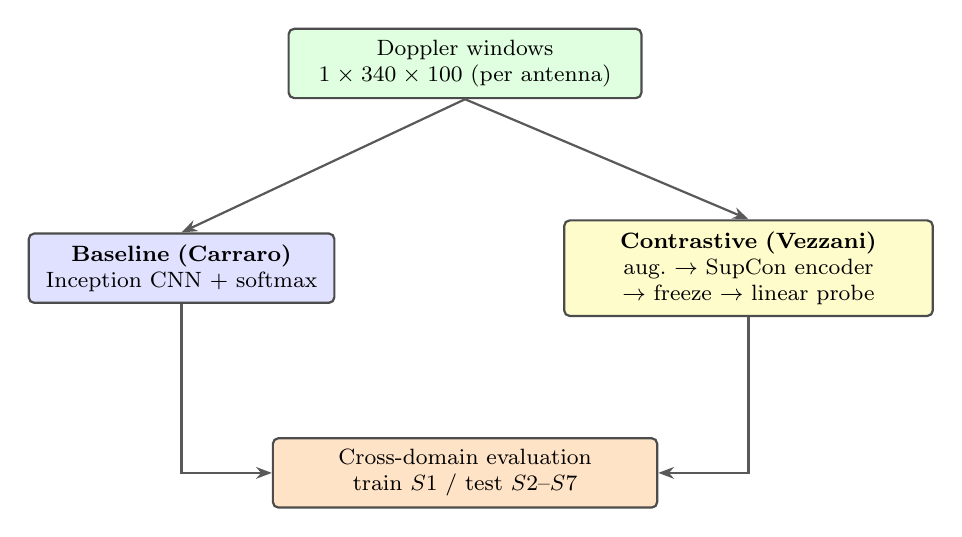
\begin{tikzpicture}[
    font=\footnotesize,
    >={Stealth[length=2mm]},
    box/.style={rectangle, rounded corners=2pt, draw=black!70, thick,
                align=center, inner sep=4pt},
    data/.style={box, fill=green!12, text width=42mm},
    base/.style={box, fill=blue!12, text width=36mm},
    cont/.style={box, fill=yellow!20, text width=44mm},
    eval/.style={box, fill=orange!22, text width=46mm},
    arr/.style={->, thick, black!65},
  ]
    \node[data] (win) at (0,0)
      {Doppler windows\\$1\times340\times100$ (per antenna)};
    \node[base] (bcnn) at (-3.6,-2.6)
      {\textbf{Baseline (Carraro)}\\Inception CNN $+$ softmax};
    \node[cont] (enc) at (3.6,-2.6)
      {\textbf{Contrastive (Vezzani)}\\aug.\ $\to$ SupCon encoder\\$\to$ freeze $\to$ linear probe};
    \node[eval] (ev) at (0,-5.2)
      {Cross-domain evaluation\\train $S1$ / test $S2$--$S7$};

    \draw[arr] (win.south) -- (bcnn.north);
    \draw[arr] (win.south) -- (enc.north);
    \draw[arr] (bcnn.south) |- (ev.west);
    \draw[arr] (enc.south) |- (ev.east);
  \end{tikzpicture}%
  }
  \caption{High-level processing pipeline. A shared front-end turns CSI traces
  into Doppler windows; the baseline chain (M.~Carraro) classifies them directly,
  while the contrastive chain (F.~Vezzani) learns an environment-invariant
  representation before a linear probe. Both are assessed with the same
  cross-domain protocol.}
  \label{fig:pipeline}
\end{figure}

\section{Signals and Features}
\label{sec:model}
\emph{(Dataset pipeline implemented by M.~Carraro.)}

\begin{figure*}[t]
  \centering
  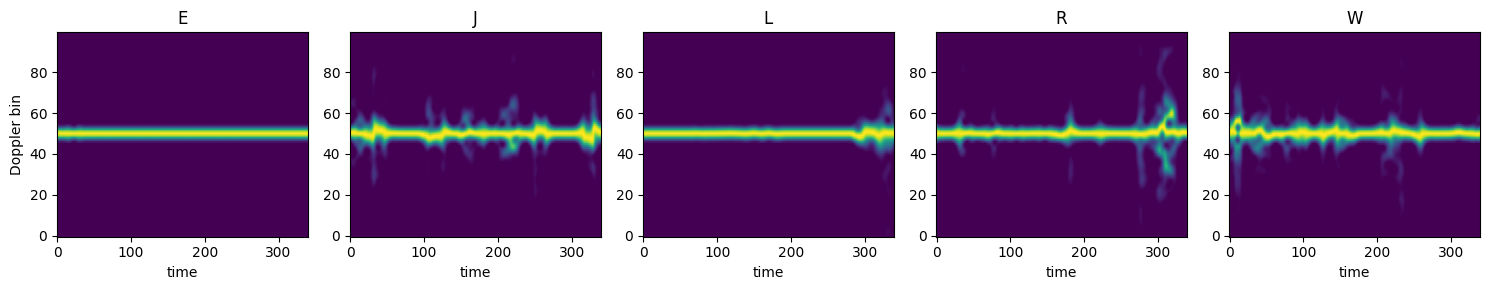
\includegraphics[width=\textwidth]{doppler_activities.png}
  \caption{One example Doppler-spectrogram window per activity (input to the
  network, transposed for readability: rows are the $100$ Doppler-velocity bins,
  columns are the $340$ time samples $\approx 2$\,s). Low-motion classes
  (\emph{empty}, \emph{sitting still}) concentrate energy around zero velocity,
  while \emph{running}/\emph{jumping} spread energy over a wide velocity range.}
  \label{fig:activities}
\end{figure*}

\subsection{The SHARP data}
We use the pre-extracted Doppler traces released with the SHARP
dataset~\cite{csidataset}, collected on IEEE~802.11ac, $80$\,MHz channels. Each
trace is a pickled array of shape $(T,100)$, where $T$ is a variable number of
time steps and $100$ is the number of Doppler-velocity bins, and corresponds to
a single receiving antenna (\texttt{stream\_1}\dots\texttt{stream\_4}) of a
four-antenna monitor.

The recordings map to seven \emph{measurement sets} $S1$--$S7$, each a distinct
(environment, monitor position, person, day) combination
(\tab{tab:conditions}). Only $S1$ is used for training; the others probe
generalization to unseen days ($S2$), unseen persons ($S3$), blocked
line-of-sight ($S4,S5$), a different room ($S6$) and the worst case of
simultaneously new room, day and person ($S7$).

\begin{table}[t]
  \centering
  \caption{Measurement sets of the SHARP dataset (after~\cite{sharp}, Table~1).
  $Mj$: monitor position; $Pi$: person; LOS: direct path present.}
  \label{tab:conditions}
  \begin{tabular}{@{}clllc@{}}
    \toprule
    Set & Monitor & Person & LOS & Role \\
    \midrule
    $S1$ & $M1$ & $P1$ & yes & \textbf{train/val/test} \\
    $S2$ & $M1$ & $P1$ & yes & test (new day) \\
    $S3$ & $M1$ & $P2$ & yes & test (new person) \\
    $S4$ & $M2$ & $P1$ & no  & test (blocked LOS) \\
    $S5$ & $M2$ & $P2$ & no  & test (blocked LOS) \\
    $S6$ & $M3$ & $P1$ & yes & test (new room) \\
    $S7$ & $M4$ & $P3$ & no  & test (all new) \\
    \bottomrule
  \end{tabular}
\end{table}

\subsection{From traces to windows}
To keep the setup comparable across \emph{all} environments, we use the five
core activities present everywhere: \textbf{E} (empty room), \textbf{J}
(jumping), \textbf{L} (sitting still), \textbf{R} (running) and \textbf{W}
(walking), matching the five-class task of the SHARP paper~\cite{sharp}. Each
trace is cut into \emph{non-overlapping} windows of $W_{\text{len}}=340$ time
samples ($\approx 2$\,s); a channel dimension is added, giving inputs of shape
$1\times 340\times 100$. Each of the four antenna streams is treated as an
independent labelled sample: the baseline is therefore a \emph{single-antenna}
classifier that never fuses information across antennas---a point we return to
in \secref{sec:results}. This yields $13{,}564$ windows, reasonably balanced
across classes (E:~$3012$, J:~$2160$, L:~$3056$, R:~$2684$, W:~$2652$).
\fig{fig:activities} shows one window per activity.

\subsection{Cross-domain split}
Following the SHARP protocol, the split is by environment, never random: the
folders of $S1$ ($S1a,S1b,S1c$) are used for training/validation and every other
set is held out for testing; a random split would leak windows from the same
person/room/day into both train and test and overestimate performance. Within
$S1$ we keep $85\%$ for training and $15\%$ for validation (stratified),
giving $2767$ / $489$ / $10{,}308$ windows for train / val / test.

\section{Learning Framework}
\label{sec:learning_framework}

\subsection{Baseline CNN (M.~Carraro)}
\label{sec:baseline}

\begin{figure*}[t]
  \centering
  \resizebox{\textwidth}{!}{%
  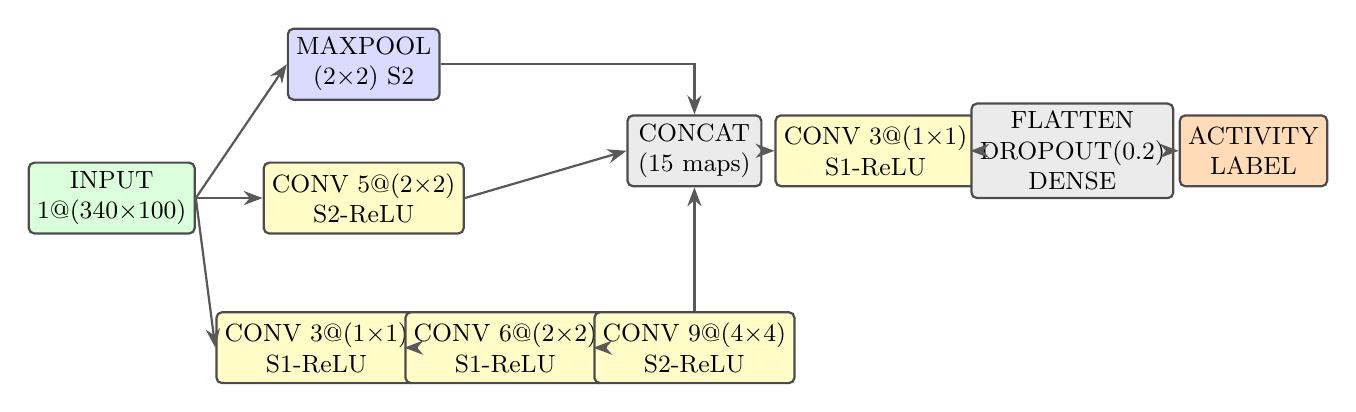
\begin{tikzpicture}[
    font=\small,
    >={Stealth[length=2.4mm]},
    box/.style={rectangle, rounded corners=2pt, draw=black!70, thick,
                align=center, minimum height=9mm, minimum width=17mm, inner sep=3pt},
    input/.style={box, fill=green!14},
    pool/.style={box, fill=blue!14},
    conv/.style={box, fill=yellow!22},
    op/.style={box, fill=black!8},
    term/.style={box, fill=orange!28},
    arr/.style={->, thick, black!65},
  ]
    % input
    \node[input] (in) at (0,0) {INPUT\\1@(340$\times$100)};
    % three branches
    \node[pool] (mp) at (3.2,1.7) {MAXPOOL\\(2$\times$2) S2};
    \node[conv] (b2) at (3.2,0.0) {CONV 5@(2$\times$2)\\S2-ReLU};
    \node[conv] (b3a) at (2.6,-1.9) {CONV 3@(1$\times$1)\\S1-ReLU};
    \node[conv] (b3b) at (5.0,-1.9) {CONV 6@(2$\times$2)\\S1-ReLU};
    \node[conv] (b3c) at (7.4,-1.9) {CONV 9@(4$\times$4)\\S2-ReLU};
    % concat + head
    \node[op]   (cat) at (7.4,0.6) {CONCAT\\(15 maps)};
    \node[conv] (red) at (9.7,0.6) {CONV 3@(1$\times$1)\\S1-ReLU};
    \node[op]   (fc)  at (12.2,0.6) {FLATTEN\\DROPOUT(0.2)\\DENSE};
    \node[term]  (lab) at (14.5,0.6) {ACTIVITY\\LABEL};

    % arrows from input to branches
    \draw[arr] (in.east) -- (mp.west);
    \draw[arr] (in.east) -- (b2.west);
    \draw[arr] (in.east) -- (b3a.west);
    % third branch chain
    \draw[arr] (b3a.east) -- (b3b.west);
    \draw[arr] (b3b.east) -- (b3c.west);
    % branches to concat
    \draw[arr] (mp.east)  -| (cat.north);
    \draw[arr] (b2.east)  -- (cat.west);
    \draw[arr] (b3c.north) -- (cat.south);
    % head
    \draw[arr] (cat.east) -- (red.west);
    \draw[arr] (red.east) -- (fc.west);
    \draw[arr] (fc.east)  -- (lab.west);
  \end{tikzpicture}%
  }
  \caption{Baseline single-antenna classification architecture (M.~Carraro), a
  faithful reproduction of the SHARP reduced-Inception module~(\cite{sharp},
  Fig.~4). Three parallel branches (max-pool / strided conv / three stacked
  convs) extract multi-scale Doppler features; the maps are concatenated
  ($1{+}5{+}9=15$), reduced to $3$ by a $1\times1$ convolution, then flattened and
  classified by a dense layer with dropout ($128{,}535$ parameters). \texttt{S2}
  denotes stride~2; every CONV is followed by a ReLU.}
  \label{fig:baseline_arch}
\end{figure*}

The baseline reproduces the simplified reduced-Inception module of SHARP
(\cite{sharp}, Fig.~4), shown in \fig{fig:baseline_arch}. Three parallel branches
process the $1\times340\times100$ input and produce feature maps of identical
spatial size $170\times50$ so they can be concatenated on the channel axis:
\begin{itemize}
  \item \textbf{Branch 1:} $\mathrm{MaxPool}(2\times2,\ \text{stride }2)$
  $\rightarrow 1$ channel (no parameters);
  \item \textbf{Branch 2:} $\mathrm{Conv}(5,\,2\times2,\ \text{stride }2)+\mathrm{ReLU}$
  $\rightarrow 5$ channels;
  \item \textbf{Branch 3:} $\mathrm{Conv}(3,\,1\times1)\rightarrow
  \mathrm{Conv}(6,\,2\times2,\ \text{pad }2)\rightarrow
  \mathrm{Conv}(9,\,4\times4,\ \text{stride }2)$, each $+\,\mathrm{ReLU}$
  $\rightarrow 9$ channels.
\end{itemize}
The branches are concatenated ($1{+}5{+}9=15$ channels), reduced to $3$ channels
by a $1\times1$ convolution, flattened, passed through $\mathrm{Dropout}(0.2)$
and a final dense layer with one logit per class. The model has
$\mathbf{128{,}535}$ trainable parameters---exactly the count reported for the
SHARP baseline CNN~\cite{sharp}.

Training uses cross-entropy loss and Adam ($\text{lr}=10^{-3}$), mini-batches of
$64$, and \emph{early stopping}: training halts when the validation loss has not
improved for $7$ epochs (budget $40$), and the best (lowest validation-loss)
weights are restored before testing. In our run, training stopped after
epoch~$13$ (best validation loss $0.993$). \fig{fig:curves} shows the loss and
accuracy curves: training accuracy keeps climbing while validation accuracy
plateaus around $0.52$---the classic signature of a model overfitting its single
training environment.

\begin{figure}[t]
  \centering
  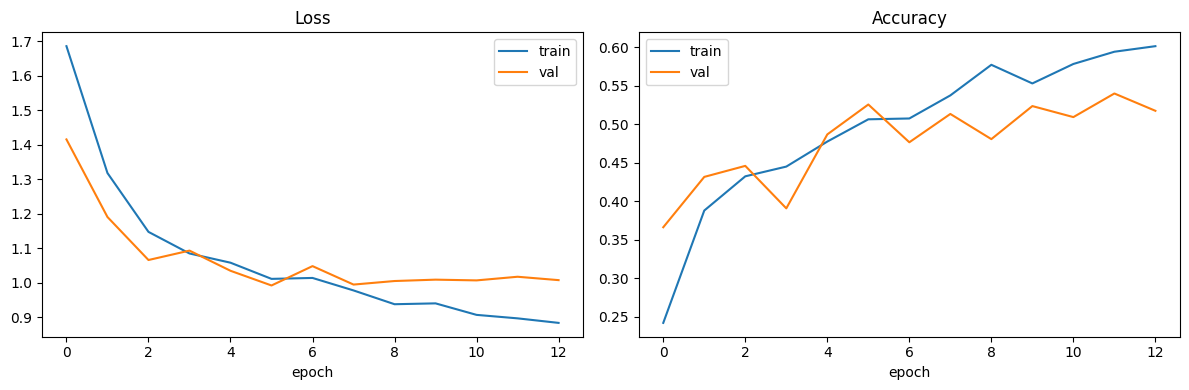
\includegraphics[width=\columnwidth]{training_curves.png}
  \caption{Baseline training. Left: cross-entropy loss; right: accuracy.
  Validation accuracy plateaus near $0.52$ while training accuracy keeps rising,
  i.e.\ the model overfits the single training set $S1$; early stopping halts
  training at epoch~13.}
  \label{fig:curves}
\end{figure}

\subsection{Contrastive extension: Supervised Contrastive Learning (F.~Vezzani)}
\label{sec:contrastive}
\emph{(Developed by F.~Vezzani; implemented and trained as Section~9 of the
notebook.)}

\subsubsection{Motivation}
The baseline is trained with plain cross-entropy on a single environment, so
nothing pushes its features to be invariant across domains. Following the
\emph{contrastive / self-supervised} direction suggested in the project
proposal, we implement \emph{Supervised Contrastive Learning}
(SupCon)~\cite{supcon}. The key change is \emph{what} is optimized: instead of
predicting the label directly, an \emph{encoder} is first trained so that two
windows of the \emph{same activity} are pulled together and windows of different
activities are pushed apart---\emph{regardless of the environment, person or
antenna they come from}. Because the objective depends only on activity
identity, the encoder is encouraged to discard environment-specific nuisances. A
tiny linear classifier is then fit on top of the frozen representation
(\emph{linear probe}).

\subsubsection{Domain-randomization augmentations}
SupCon needs, for each window, two augmented ``views'' that keep the activity
intact but perturb nuisance factors, acting as a light domain randomization
(\fig{fig:aug}). All transforms run on-GPU on a whole batch (default
parameters in parentheses):
\begin{itemize}
  \item \textbf{amplitude scaling} by a per-window random gain
  ($\mathcal{U}(0.8,1.2)$)---rooms/distances reflect the signal with different
  strength;
  \item \textbf{additive Gaussian noise} ($\sigma=0.05$);
  \item \textbf{circular time shift} ($\pm 40$ samples)---the activity does not
  depend on where in the $\approx 2$\,s window it starts;
  \item \textbf{time and Doppler masking} (SpecAugment-style: a zeroed band of
  $40$ time samples and $15$ velocity bins)---forces the encoder to use the whole
  time--velocity pattern rather than any single region.
\end{itemize}

\begin{figure}[t]
  \centering
  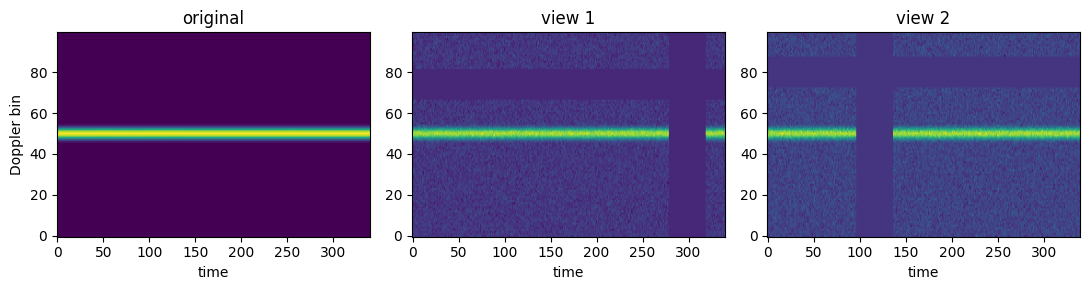
\includegraphics[width=\columnwidth]{augment_views.png}
  \caption{A window (\emph{left}) and two augmented views. Amplitude scaling and
  Gaussian noise change the texture; the circular time shift and the
  SpecAugment-style time/Doppler masks (dark bands) hide parts of the pattern,
  while the activity signature (the horizontal energy band) is preserved.}
  \label{fig:aug}
\end{figure}

\subsubsection{Encoder and projection head}
The encoder $f(\cdot)$ is a deeper, batch-normalized evolution of the baseline's
Inception block (\tab{tab:encoder}). It keeps the three-branch Inception
front-end (max-pool / strided conv / deeper conv, concatenated to $41$ channels)
but adds (i) batch normalization after every convolution, (ii) a $1\times1$
channel-mixing reduction to $32$ channels, (iii) a second downsampling stage
($32\!\rightarrow\!64\!\rightarrow\!128$), and (iv) \emph{global average
pooling}, replacing the baseline's large \texttt{flatten}$\rightarrow$dense layer
with a fixed $128$-dimensional representation $h$ that has fewer parameters and
is more shift-robust. A small MLP \emph{projection head} $g(\cdot)$
($128\!\rightarrow\!128\!\rightarrow\!128$, ReLU) maps $h$ to an
$L_2$-normalized embedding $\bm{z}=g(h)$ on the unit hypersphere; as prescribed by
SupCon, the loss is applied to $\bm{z}$ and the head is \emph{discarded} after
pre-training, so classification uses $h$. The whole model has $130{,}952$
parameters (encoder $\approx\!97.9$k $+$ head $\approx\!33$k), comparable to the
baseline's $128.5$k.

\begin{table}[t]
  \centering
  \caption{Contrastive encoder $f(\cdot)$; output sizes for a
  $1\times340\times100$ input. BN$+$ReLU follow every convolution; ``sN''
  denotes stride~N (default stride~1). The pooling output is the $128$-d
  representation $h$.}
  \label{tab:encoder}
  \setlength{\tabcolsep}{4pt}
  \begin{tabular}{@{}lll@{}}
    \toprule
    Stage & Layers & Output ($C\times H\times W$) \\
    \midrule
    Inception & maxpool(2); conv(16,s2); & $41\times170\times50$\\
              & conv(16)$\rightarrow$conv(24,s2) & \\
    Reduce    & conv(32,\,$1\times1$) & $32\times170\times50$\\
    Stage 2   & conv(64,s2)$\rightarrow$conv(128,s2) & $128\times43\times13$\\
    Pool      & global average pool & $128$\\
    \bottomrule
  \end{tabular}
\end{table}

\subsubsection{SupCon loss}
For a batch of $L_2$-normalized embeddings with labels, each anchor $i$ attracts
every other sample sharing its label (its positive set $P(i)$) and repels all
others, through a temperature-scaled softmax over cosine similarities:
\begin{equation}
\label{eq:supcon}
\mathcal{L}=\frac{1}{|I|}\sum_{i\in I}\frac{-1}{|P(i)|}\sum_{p\in P(i)}
\log\frac{\exp(\bm{z}_i\!\cdot\!\bm{z}_p/\tau)}
{\sum_{a\neq i}\exp(\bm{z}_i\!\cdot\!\bm{z}_a/\tau)},
\end{equation}
where $I$ is the set of anchors with at least one same-class positive (the
implementation averages the per-anchor terms over the batch) and the temperature
is $\tau=0.07$. Unlike self-supervised SimCLR~\cite{simclr}, using the labels in
\eq{eq:supcon} makes \emph{all} same-activity windows in the batch positives---even
those from different files or environments---which turns generic contrastive
learning into an environment-invariant \emph{activity} representation.

\subsubsection{Training and evaluation protocol}
Everything uses the \emph{same} $S1$-based split as the baseline.
\begin{itemize}
  \item \textbf{Contrastive pre-training.} Each batch is expanded into two
  augmented views; encoder and head are trained jointly with Adam
  (lr~$10^{-3}$, weight decay~$10^{-4}$) for up to $30$ epochs with early
  stopping (patience~$7$) on the validation contrastive loss, keeping the best
  encoder.
  \item \textbf{Linear probe.} The encoder is frozen, embeddings are
  pre-computed and standardized with training statistics, and a single
  $\mathrm{Linear}(128,5)$ layer is trained with cross-entropy (Adam,
  lr~$10^{-3}$, early stopping). This isolates the quality of the representation.
  \item \textbf{Optional fine-tuning.} The encoder is then unfrozen and the full
  network fine-tuned end-to-end with a small learning rate ($10^{-4}$).
\end{itemize}
The model is evaluated under the same cross-domain protocol as the baseline
(train on $S1$, test on $S2$--$S7$). A t-SNE projection of the test embeddings,
colored by activity and by environment, is used as a diagnostic of
environment-invariance.


% !TEX root = report.tex

\section{Results}
\label{sec:results}

All numbers come from the stored notebook outputs, one run per configuration,
under the same protocol: train on $S1$, test on the unseen $S2$--$S7$.
\tab{tab:compare} collects them per measurement set and \fig{fig:perset} plots
the four milestones; \tab{tab:versions} maps each column to the change that
produced it.

\subsection{Baseline}
On the pooled unseen test set the baseline reaches $\mathbf{48.2\%}$ accuracy
(test loss $1.052$), from $45.5\%$ ($S2$) to $52.3\%$ ($S7$). Its confusion matrix
(\fig{fig:cm}\,(a)) shows two dominant error modes: \emph{sitting still} is
absorbed by \emph{empty} ($L\!\rightarrow\!E$: $0.76$), both being near-static and
concentrated at zero Doppler velocity, and \emph{running}/\emph{walking} are
heavily confused with each other ($0.39$ and $0.28$).

\subsection{Contrastive representation}
The linear probe on the frozen SupCon encoder raises overall accuracy to
$\mathbf{53.1\%}$ (validation $58.3\%$): $+4.9$ points, and an improvement on
\emph{every} set, the largest on $S3$ ($+8.3$, unseen person) and $S7$ ($+5.9$,
all conditions new). Its confusion matrix (\fig{fig:cm}\,(b)) sharpens
\emph{running} and softens the $L\!\rightarrow\!E$ confusion
($0.76\!\rightarrow\!0.52$). \emph{End-to-end fine-tuning} then \emph{hurts},
dropping back to $48.4\%$: freezing the pre-trained encoder is what generalizes,
while fine-tuning re-overfits the single training environment.

The t-SNE projection (\fig{fig:tsne}, from the sliding-window run of
\secref{sec:sliding}) is the most informative diagnostic. Colored by
\emph{environment} (right) the points are thoroughly mixed---the
SupCon objective \emph{did} reach its design goal of an environment-invariant
representation. Colored by \emph{activity} (left) the space splits into a
static region (\emph{empty}, \emph{sitting}) and a moving arc (\emph{jumping},
\emph{running}, \emph{walking}), but the activities \emph{within} each region
stay partly entangled: contrastive learning removed the \emph{domain} nuisance
and exposed a harder, intrinsic limit---a single-antenna $\approx\!2$\,s window
does not fully separate the activities, whichever way it is encoded.
Consistently, in both runs the SupCon loss fell only from $\approx\!4.6$ to
$\approx\!4.3$: the pre-training never fully converged.

\begin{figure*}[t]
  \centering
  \begin{subfigure}{0.245\textwidth}
    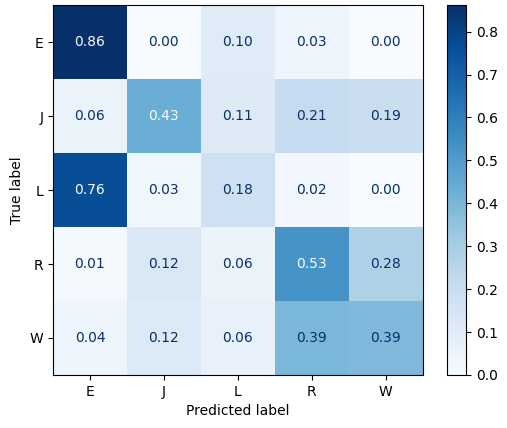
\includegraphics[width=\textwidth]{confusion_overall_c.png}
    \caption{baseline, non-overlapping}
  \end{subfigure}\hfill
  \begin{subfigure}{0.245\textwidth}
    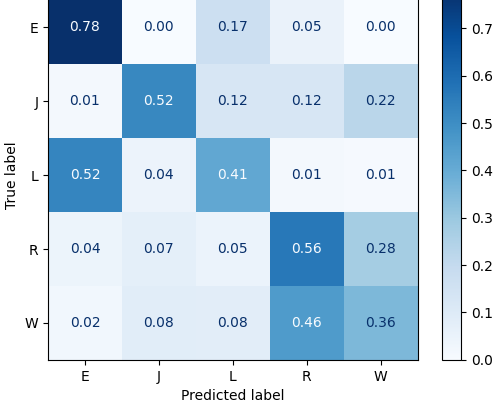
\includegraphics[width=\textwidth]{cl_confusion_c.png}
    \caption{$+$ SupCon linear probe}
  \end{subfigure}\hfill
  \begin{subfigure}{0.245\textwidth}
    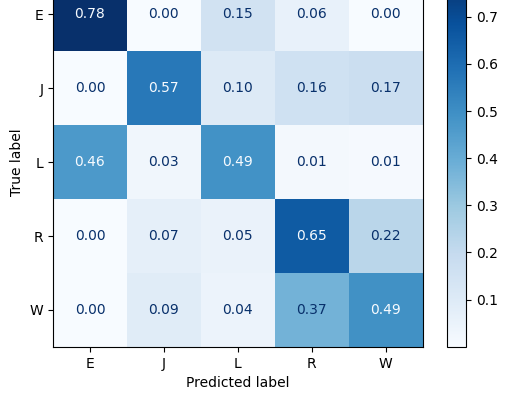
\includegraphics[width=\textwidth]{confusion_v4_single_c.png}
    \caption{baseline, sliding window}
  \end{subfigure}\hfill
  \begin{subfigure}{0.245\textwidth}
    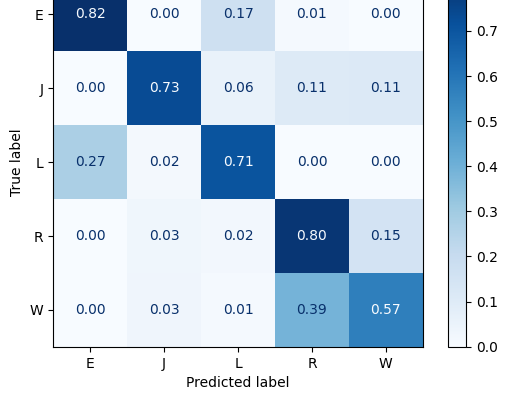
\includegraphics[width=\textwidth]{confusion_v4_fused_c.png}
    \caption{$+$ $4$-antenna fusion}
  \end{subfigure}
  \caption{Row-normalized confusion matrices on all unseen test environments,
  along the four milestones of \fig{fig:perset}. The contrastive representation
  (b) softens the $L\!\rightarrow\!E$ confusion of the baseline (a); the sliding
  window (c) lifts every class; fusion (d) then repairs the low-motion pair
  itself, $L$ going from $0.50$ to $0.75$ correct with the \emph{same} weights.}
  \label{fig:cm}
\end{figure*}

\begin{figure}[t]
  \centering
  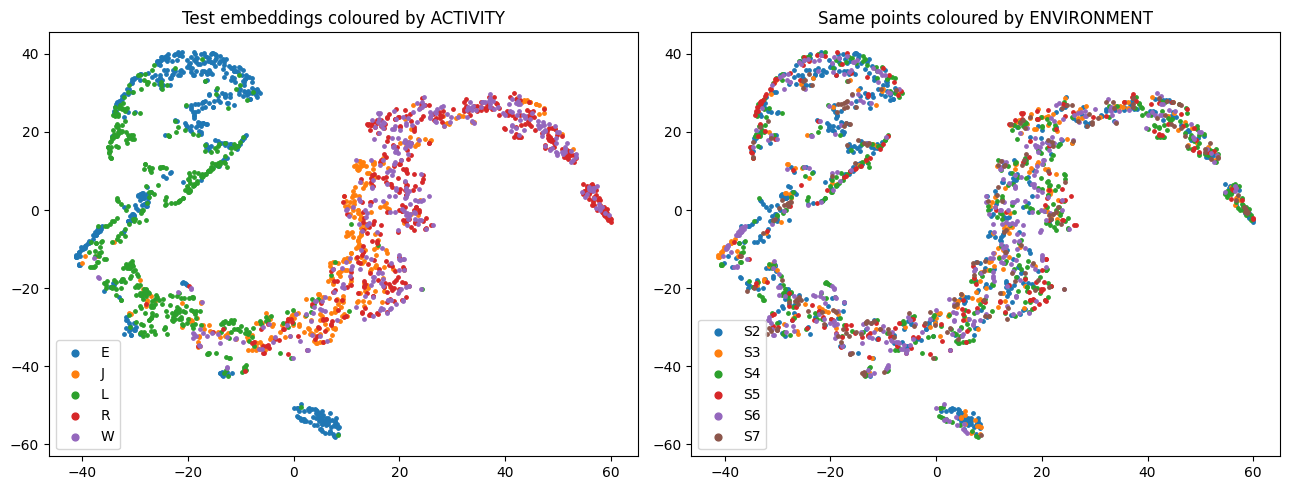
\includegraphics[width=\columnwidth]{tsne_slide.png}
  \caption{t-SNE of the test embeddings of the SupCon encoder (sliding-window
  run). \emph{Left},
  colored by activity: a static region (\emph{empty}, \emph{sitting}) and a
  moving arc (\emph{jumping}, \emph{running}, \emph{walking}). \emph{Right}, the
  same points colored by environment: the colors are mixed \emph{inside} the
  structure, i.e.\ the space is organized by \emph{activity}, not by
  \emph{environment}.}
  \label{fig:tsne}
\end{figure}

\subsection{Optimizer schedule}
The slow schedule changes only the learning rate, the patience and the epoch
budget, so the two runs isolate that factor. Slowing
training down \emph{improves} cross-domain accuracy from $48.2\%$ to $51.3\%$
($+3.1$ points, five sets out of six) even though the model fits its own training
data \emph{worse} ($0.575$ vs.\ $0.601$, \fig{fig:curves}). With a single
training environment the two objectives conflict: an epoch spent fitting $S1$
better is also an epoch spent memorizing its room, person and day. It also
tempers the previous subsection---$+3.1$ of the contrastive model's $+4.9$ points
can be bought with an optimizer setting alone, so single-run gains of a few
points here are fragile.

\subsection{Sliding-window front-end}
\label{sec:sliding}
Cutting the same recordings at stride $30$ instead of $340$ turns $13{,}564$
windows into $152{,}320$ and takes the \emph{unchanged} architecture from
$48.2\%$ to $\mathbf{59.3\%}$ ($+11.1$ points), improving every measurement set
by $8.4$ to $15.3$ points. Two caveats keep this honest: the run also raises the
early-stopping patience from $7$ to $12$, so a small part of the gain belongs to
the longer schedule; and the extra windows are strongly
correlated, so the effective sample size grows far less than tenfold. The cost is
real---$\approx\!21$\,GB of resident memory and an epoch an order of magnitude
slower, which is exactly why the loader had to allocate once instead of
concatenating---but the payoff is the single largest gain from the data side, and
it confirms that the reference implementation's stride is not an arbitrary
choice. \fig{fig:curves}(c) shows the model now reaching $0.756$ training
accuracy with validation accuracy $12$ points above the non-overlapping run, i.e.\
the denser windows buy genuine fitting capacity rather than only noise.

\subsection{Multi-antenna decision fusion}
Averaging the four per-antenna probability vectors (\eq{eq:fusion}) is the
largest single improvement we measured, and it is free: no retraining, no extra
parameters, one softmax and one group-average at inference. On the
sliding-window model it lifts $59.3\%$ to $\mathbf{72.1\%}$ ($+12.8$ points, from
$+6.9$ on $S7$ to $+17.1$ on $S2$); on the non-overlapping model it gave $+10.2$
($51.3\!\rightarrow\!61.5\%$). The gain is therefore robust to the data regime.

Its mechanism, though, changes with that regime. At stride $340$
(\tab{tab:compare}) fusion sharpened the motion classes but left
\emph{sitting}$\rightarrow$\emph{empty} untouched: with almost no motion in a
window the four antennas simply agreed on the same wrong answer. At stride $30$
the single-antenna model is already half-right on that pair
(\fig{fig:cm}\,(c), $L$ at $0.50$), and fusion converts it into the largest
per-class gain of all---$L$ reaches $0.75$ and $L\!\rightarrow\!E$ falls from
$0.45$ to $0.23$ (\fig{fig:cm}\,(d))---alongside \emph{jumping}
($0.56\!\rightarrow\!0.72$) and \emph{running} ($0.63\!\rightarrow\!0.75$).
Averaging only helps where the individual antennas disagree; denser temporal
coverage is what creates that disagreement on low-motion windows.

\begin{figure}[t]
  \centering
  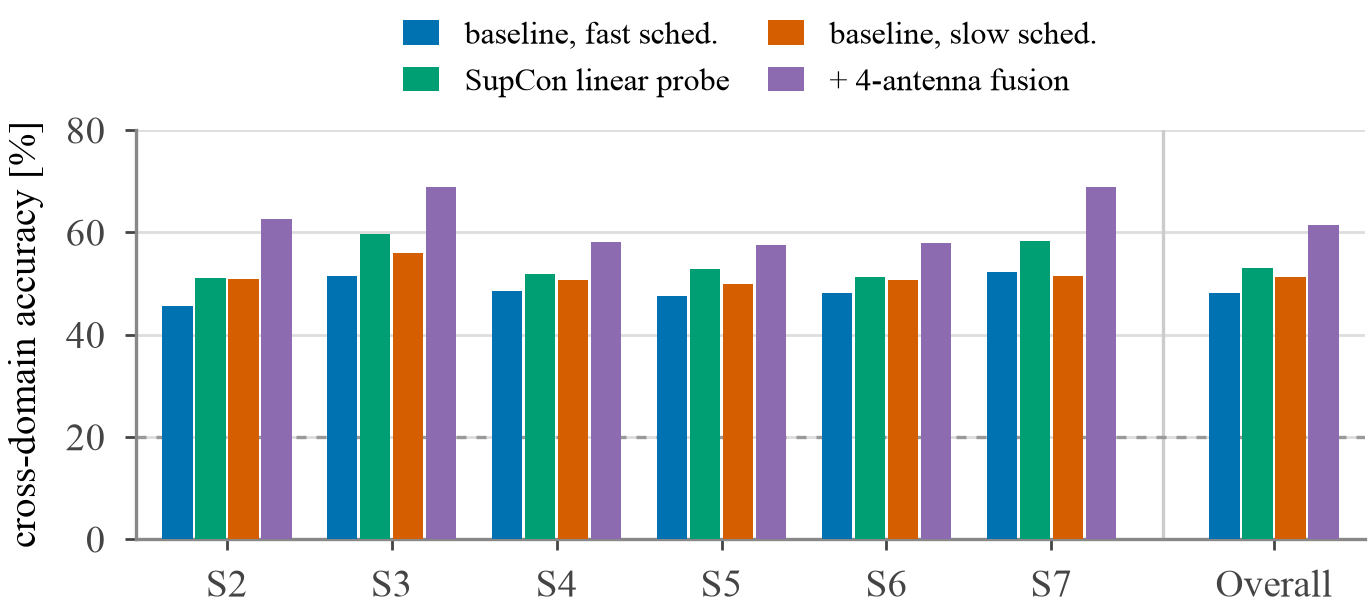
\includegraphics[width=\columnwidth]{perset_accuracy.png}
  \caption{Cross-domain accuracy per measurement set along the four milestones
  (dashed line: the $20\%$ chance level). Every unseen set benefits from the
  sliding window and, on top of it, from antenna fusion.}
  \label{fig:perset}
\end{figure}

\subsection{Does contrastive learning still help?}
Repeating the contrastive stage on the sliding-window data answers a question the
first experiment could not: the linear probe now reaches $58.3\%$, i.e.\ $1.0$
point \emph{below} the plain baseline it beat by $4.9$ points in the data-poor
regime, and fine-tuning again does worse ($57.0\%$). Read together with
\tab{tab:compare}, the contrastive stage behaves as a \emph{data-efficiency}
mechanism rather than a domain-invariance mechanism per se: when only $2767$
training windows are available it buys a representation that plain cross-entropy
cannot learn, and when $31{,}103$ (correlated) windows are available
cross-entropy catches up on its own. One confound deserves mention: the
contrastive and probe learning rates were left at $10^{-4}$ in that run while the
baseline used $10^{-3}$, so part of the one-point deficit may be an under-trained
encoder rather than the data regime.

\subsection{Comparison with the SHARP paper}
\tab{tab:compare} places our results next to the SHARP paper~\cite{sharp}: the
\emph{full} system (strongest-path sanitization $+$ 4-antenna fusion) and an
\emph{ablation} that swaps the strongest-path sanitization for the standard
reference-antenna method, feeding the \emph{same} CNN (\cite{sharp}, Table~4).
Full SHARP stays above $95\%$ everywhere. Our best configuration
(sliding window $+$ fusion, $72.1\%$) beats the ablation on \emph{every} unseen
set, by $10.6$ points ($S7$) to $26.8$ points ($S5$), and its margin is largest
exactly where the ablation collapses---the blocked-line-of-sight sets $S4$ and
$S5$. The residual $\sim\!26$-point gap to full SHARP is thus concentrated in the
one ingredient we do not implement, the strongest-path phase sanitization. The
acquisition campaigns behind the dataset also spanned nearly two years
(\cite{sharp}, Sec.~5.2), and that time diversity is itself part of what the
reference results build on.

\begin{table*}[t]
  \centering
  \caption{Per-set accuracy (\%), training on $S1$ and testing on the unseen
  sets, one run per column. Non-overlapping windows: baseline under the fast
  ($10^{-3}$) and slow ($10^{-4}$) schedules, SupCon linear probe, and fusion on
  the slow-schedule model. Sliding window (stride $30$): baseline, SupCon probe
  and fusion. Fusion always re-uses the weights of the baseline to its left.
  SHARP columns from~\cite{sharp} (Tables~3 and~4).}
  \label{tab:compare}
  \setlength{\tabcolsep}{5pt}
  \small
  \begin{tabular}{@{}lcccccccccc@{}}
    \toprule
     & \multicolumn{4}{c}{\textbf{Non-overlapping windows}}
     & \multicolumn{3}{c}{\textbf{Sliding window (stride 30)}}
     & \multicolumn{2}{c}{\textbf{SHARP~\cite{sharp}}}\\
    \cmidrule(lr){2-5}\cmidrule(lr){6-8}\cmidrule(lr){9-10}
    Set & Base (fast) & SupCon & Base (slow) & $+$ Fusion
        & Base & SupCon & $+$ Fusion & Full & Abl.\\
    \midrule
    $S2$ & $45.5$ & $51.1$ & $50.9$ & $62.6$ & $60.8$ & $59.3$ & $77.9$ & $99.8$ & $59.8$\\
    $S3$ & $51.4$ & $59.7$ & $55.9$ & $68.8$ & $61.6$ & $61.5$ & $75.2$ & $99.3$ & $58.0$\\
    $S4$ & $48.5$ & $51.9$ & $50.6$ & $58.1$ & $56.9$ & $55.6$ & $66.2$ & $97.6$ & $43.5$\\
    $S5$ & $47.5$ & $52.9$ & $49.8$ & $57.5$ & $57.4$ & $55.3$ & $66.0$ & $96.6$ & $39.2$\\
    $S6$ & $48.1$ & $51.3$ & $50.6$ & $57.9$ & $57.4$ & $56.5$ & $72.7$ & $99.8$ & $59.4$\\
    $S7$ & $52.3$ & $58.2$ & $51.5$ & $68.9$ & $64.0$ & $65.3$ & $70.9$ & $96.0$ & $60.3$\\
    \midrule
    \textbf{Overall} & $48.2$ & $53.1$ & $51.3$ & $61.5$ & $59.3$ & $58.3$ &
    $\mathbf{72.1}$ & $\sim\!98$ & $\sim\!53$\\
    \bottomrule
  \end{tabular}
\end{table*}

\subsection{Discussion}
\label{sec:discussion}

\paragraph{What each change bought}
Ranked by measured effect, decision fusion ($+12.8$) and the sliding window
($+11.1$) dominate the contrastive representation ($+4.9$, and $-1.0$ once data
is plentiful) and the optimizer schedule ($+3.1$). The ordering is a finding in
itself: the two cheapest changes---a stride constant and a few lines of
post-processing over information already present in the dataset---beat the one
that cost the most design effort, and they compose, taking the \emph{same}
$128{,}535$-parameter network from $48.2\%$ to $72.1\%$. It also matches SHARP's
own ablation, where accuracy grows monotonically with the number of fused
antennas~\cite{sharp}.

\paragraph{Why we are still far from SHARP}
The gap is now essentially one component. SHARP uses the \emph{strongest}
multipath component as phase reference, and its ablation shows the standard
reference-antenna method makes the \emph{same} CNN collapse from $>95\%$ to
$39$--$60\%$ (\tab{tab:compare}, last column). Our best model sits $10$ to $27$
points \emph{above} that ablation, so we have reproduced the decision-level half of
SHARP's robustness and improved on the data side, but none of its
signal-processing half. Training on one small environment also makes every number
high-variance.

\paragraph{Where representation learning fits}
The SupCon stage attacks domain shift on the \emph{representation} axis and, as
the t-SNE shows, succeeds there; but its measured advantage evaporates when the
front-end supplies ten times more windows. The practical reading is that
contrastive pre-training is worth its complexity when labelled windows are
scarce---which is the realistic setting for a new deployment with one calibration
environment---while in the data-rich regime the effort is better spent on the
front-end and on the decision rule. The experiment left undone is fusion on top
of the frozen probe with the contrastive stage re-tuned at $10^{-3}$: all the
components exist in the released code, but no run combines them.


% !TEX root = report.tex

\section{Concluding Remarks}
\label{sec:conclusions}

We reproduced and evaluated a baseline Wi-Fi HAR pipeline under a strict
cross-domain protocol ($48.2\%$ on unseen environments) and added a Supervised
Contrastive Learning extension that improves cross-domain accuracy on every
measurement set ($53.1\%$ overall, $+4.9$ points). A t-SNE analysis shows that
the extension achieves its intended goal---an environment-invariant
representation---while a direct comparison with the SHARP paper~\cite{sharp}
places both models well below the full pipeline, whose multi-antenna decision
fusion and strongest-path phase sanitization we do not implement.

The practical value of the extension is that it recovers domain robustness
\emph{on the learning side}, with a lightweight encoder, no extra
signal-processing, and a frozen, reusable feature space. Since its residual
errors are \emph{activity} confusions rather than \emph{domain} shift, the
contrastive encoder is complementary to SHARP's antenna fusion: the clearest next
step is to combine the two---keeping the frozen encoder---ideally with a
sliding-window dataset and multi-seed runs.

\paragraph{What we learned and difficulties encountered}
The main lesson was that a strict, environment-based split changes the story:
modest-looking numbers ($\sim\!50\%$) are the honest cost of never seeing the
test environment, which a random split would have hidden. The t-SNE proved
valuable as a diagnostic---it revealed that contrastive learning had solved the
\emph{domain} axis but not the \emph{activity} axis. The main difficulties were:
(i) getting SupCon pre-training to converge (the loss barely moved), so the
representation is useful but under-trained; (ii) the counter-intuitive finding
that end-to-end fine-tuning \emph{hurt} generalization by re-overfitting the
single environment, which taught us to trust the frozen-encoder / linear-probe
evaluation; and (iii) the high run-to-run variance of the small baseline, which
makes single-run comparisons fragile and calls for multi-seed averaging.


%=============================================================================
\bibliography{biblio}
\bibliographystyle{ieeetr}

\end{document}
